\documentclass[]{article}
\usepackage{xeCJK}
\usepackage{changepage}
\usepackage{tikz}
\usepackage{amsmath}

\tikzset{elegant/.style={smooth,thick,samples=50,cyan}}
\tikzset{eaxis/.style={->,>=stealth}}

%opening
\title{Computer Networking: A Top-Down Approach \\ Homework 1}
\author{Class 42 \\ 欧阳鹏程 \\ 2141601030 \\ Copyright Notice: BY-NC-SA}

\begin{document}

\maketitle


\section{Addtional problems}

\begin{enumerate}
	\item 
	Explain precisely following abbreaviations:
	\begin{itemize}
		\subitem
		TCP,
		HTTP,
		SMTP,
		DNS,
		FTP,
		ATM,
		ISDN,
		ADSL,
		HFC,
		ISP,
		WAP,
		LAN,
		WAN,
		MAN,
		WLAN,
		ISO,
		OSI
	\end{itemize}

	\paragraph{A.}
	TCP: Transmission Control Protocol, which is the Internet's transport-layer, connection-oriented, reliable transport protocol, says the two processes must first "handshake" with each other before one application process can begin to send data to another.
	
	\begin{adjustwidth}{0.05cm}{0cm}
		\qquad HTTP: HyperText Transfer Protocol, the Web's application-layer protocol, defines the structure of the messages exchanging between client program and server programs.
		
		\qquad SMTP: Simple Mail Transfer Protocol is the principal application-layer protocol for Internet electronic mail, transferring messages from senders' mail servers to the recipients' mail servers.
		
		\qquad DNS: Domain Name System is a distributed database implemented in a hierarchy of DNS servers and an application-layer protocol that allows hosts to query the distributed database to translate user-supplied hostnames to IP addresses.
		
		\qquad FTP: File Transfer Protocol is used for transferring files on the Internet.
		
		\qquad ATM: Asynchronous Transfer Mode is a fast transferring mode that designed for grouping and exchanging.
		
		\qquad ISDN: Integrated Services Digital Network is a international network digital telephone standard.
		
		\qquad ADSL: Asymmetric Digital Subscriber Line means that the uploading rate and the downloading rate is not the same.
		
		\qquad HFC: Hybrid Fiber-coxial Cable is a telecommunications industry term for a broadband network that combines optical fiber and coaxial cable.
		
		\qquad ISP: Internet Service Providers is in itself a network of packet switches and communication links and provide a variety of types of network access to the end system and Internet access to content providersm connecting Web sites directly to the Internet.
		
		\qquad WAP: Wireless Application Protocol, a secure specification that allows users to access information instantly via handheld wireless devicessuch as mobile phones, pagers, two-way radios, smartphones and communicators.
				
		\qquad LAN: Local Area Network is a network covering partial area.
		 
		\qquad WAN: Wide Area Network is a network connecting a series of different LANs in different regions, used for communication of computer.
		
		\qquad MAN: Metropolitan Area Network is a big network who ranges between LAN and WAN.
		
		\qquad WLAN: Wireless Local Area Networks uses radio frequency instead of coaxial to form a local area network.
		
		\qquad ISO: Internatioal Organization for Standardization is an organizarion formulating several standards over the world.
		
		\qquad OSI: Open Systems Interconnection is a conceptual model that characterizes and standardizes the communication functions of a telecommunication or computing system without regard to their underlying internal structure and technology.
	\end{adjustwidth}

	\item
	Explain following concepts:
	\subitem
	TCP/IP
	\subitem
	Circuit switching,
	Packet switching,
	Message switching,
	Virtual circuit
	
	\paragraph{A.}
	TCP/IP: The Internet's principal protocols are collectively known as TCP/IP.
	\begin{adjustwidth}{0.1cm}{0cm}
		\qquad Circuit switching: Circuit switching is an approach to moving data through a network of links and switches where the resources needed aling a path to provide for communication between the end-systems.
	
		\qquad Packet switching: Packet switching is an approach to moving data through a network of links and switches where the resources are not reserved. As a consequence, the end-system may have to wait for access to a communication link.
		
		\qquad Message switching: An approach to moving data where the entire message will be sent at one time.
		
		\qquad Virtual circuit: A virtual circuit is a means of transporting data over a \textbf{packet switched} computer network in such a way that it appears as though there is a dedicated physical layer link between the source and destination end systems of this data. 
	\end{adjustwidth}
\end{enumerate}

\section{Problems on textbook}
\subsection{Review questions}

\begin{enumerate}
	\item[R11.]
	Suppose there is exactly one packet switch between a sending host and a
	receiving host. The transmission rates between the sending host and the
	switch and between the switch and the receiving host are R1 and R2, respectively. Assuming that the switch uses store-and-forward packet switching,
	what is the total end-to-end delay to send a packet of length L? (Ignore
	queuing, propagation delay, and processing delay.)
	
	\paragraph{A.}
	There are totally four types of delay: Processing delay, Queuing delay, \textbf{Transmission delay} and Propagation delay. Ignoring those mentioned three delays, we just need to consider only one type of delay: Transmission delay.

	\begin{center}
		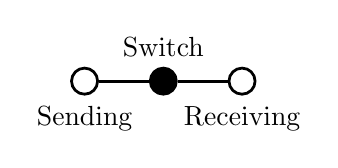
\begin{tikzpicture}[line width = 1pt,
		solid/.style = {circle, draw, fill = black, minimum size = 0.3cm},
		empty/.style = {circle, draw, fill = white, minimum size = 0.3cm}]
		
		\node [empty, label = below:Sending] (A) at (1,1) {};
		\node [empty, label = below:Receiving] (B) at (3,1) {};
		\node [solid, label = above:Switch] (C) at (2,1) {};
	
		\draw (A) -- (C);
		\draw (B) -- (C);
		
		\end{tikzpicture}
	\end{center}

	So:
	\[ 
		T = t_{transmission} = \dfrac{L}{R_{1}} + \dfrac{L}{R_{2}}
	\]

	\item[R12.]
	What advantage does a circuit-switched network have over a packet-switched
	network? What advantages does TDM have over FDM in a circuit-switched
	network?
	
	\paragraph{A.}
	\begin{itemize}
		\item There are mainly two advantages a circuit-switched network have over a packet-switched network:
		\begin{adjustwidth}{0.3cm}{0cm}
			\begin{enumerate}
				\item There being a real physical route, the delay is tiny compared with the delay in packet-switched network. 
				
				\item The sequence of message the receiving host gets will keep the same as it being sent.
			\end{enumerate}
		\end{adjustwidth}
	
		\item As for the advantage TDM has over FDM, it is obvious that TDM can \textbf{support many more users} one time than FDM can.
	\end{itemize}
	
	\item[R14.]
	Why will two ISPs at the same level of the hierarchy often peer with each
	other? How does an IXP earn money?
	
	\paragraph{A.}
	By peering with each other directly, the two ISPs can reduce their payments to their provider ISPs. An Internet Exchange Points is a meeting point where multiple ISPs can connect and/or peer together. An ISP earns its money by charging each of the ISPs that connect to the IXP a relatively small fee, which may depend on the amount of traffic sent to or received from the IXP.
	
	\item[R19.]
	Suppose Host A wants to send a large file to Host B. The path from Host A to
	Host B has three links, of rates $R_{1}$ = 500 kbps, $R_{2}$ = 2 Mbps, and $R_{3}$ = 1 Mbps.
	
	a. Assuming no other traffic in the network, what is the throughput for the
	file transfer?
	
	b. Suppose the file is 4 million bytes. Dividing the file size by the throughput,
	roughly how long will it take to transfer the file to Host B?
	
	c. Repeat (a) and (b), but now with $R_{2}$ reduced to 100 kbps.
	
	\paragraph{A.}
	\begin{enumerate}
		\item[a.] $Throughput =  \min\{R_{1}, R_{2}, R_{3}\} = R_{2} = 500 kbps $
		\item[b.] $Transfer time = \dfrac{file size}{throughput} = \dfrac{4 \times 10^{6}}{500 \times 10^{3}}s = 64 s$
		\item[c.] $Throughput = \min\{R_{1}, R_{2}, R_{3}\} = R_{2} = 100 kbps
		\\
		Transfer time = \dfrac{file size}{throughput} = \dfrac{4 \times 10^{6}}{100 \times 10^{3}}s = 320 s$
	\end{enumerate}
		
	\subsection{Problems}
	\item[P5.]
	Review the car-caravan analogy in Section 1.4. Assume a propagation speed
	of 100 km/hour.
	
	a. Suppose the caravan travels 150 km, beginning in front of one tollbooth,
	passing through a second tollbooth, and finishing just after a third tollbooth. What is the end-to-end delay?
	
	b. Repeat (a), now assuming that there are eight cars in the caravan instead
	of ten.
	
	\paragraph{A.}
	\begin{enumerate}
		\item[a.] 
		\begin{equation}
			\begin{split}
				Delay & = d_{propagation} + d_{transmission} \\ & = 10 \times 12 s \times 3 + \dfrac{150}{100} h \\ & = 96 minutes
			\end{split}
		\end{equation}
		
		\item[b.] 
		\begin{equation}
			\begin{split}
				Delay & = d_{propagation} + d_{transmission} \\ & = 8 \times 12 s \times 3 + \dfrac{150}{100} h \\ & = 94 minutes 48 seconds
			\end{split}
		\end{equation}
	\end{enumerate}
	
	\item[P12.]
	A packet switch receives a packet and determines the outbound link to which
	the packet should be forwarded. When the packet arrives, one other packet is
	halfway done being transmitted on this outbound link and four other packets
	are waiting to be transmitted. Packets are transmitted in order of arrival.
	Suppose all packets are 1,500 bytes and the link rate is 2 Mbps. What is the
	\textbf{queuing delay} for the packet? More generally, what is the queuing delay
	when all packets have length L, the transmission rate is R, x bits of the
	currently-being-transmitted packet have been transmitted, and n packets are
	already in the queue?
	
	\paragraph{A.}
	There are 4.5 packets are waiting to be transmitted before the last bit in the last packet, so the queuing delay should be:
	\begin{equation}
		\begin{split}
			Delay & = \dfrac{4.5 \times 1500 \times 8}{2 \times 10^{6}}s \\ & = 0.027 s;
		\end{split}
	\end{equation}
		
		More generally, there remains $n \times L + L - x$ bits waiting to be transported before the last bit in the queue. Consequently:
	\[
		Delay = \dfrac{n \times L + L - x}{R} s
	\]	 
	
	\item[P14.]
	Consider the queuing delay in a router buffer. Let $ I $ denote traffic intensity;
	that is, $ I = \dfrac{La}{R} $. Suppose that the queuing delay takes the form $ \dfrac{IL}{R (1 – I)} $
	for $ I < 1 $.
	
	a. Provide a formula for the total delay, that is, the queuing delay plus the
	transmission delay.
	
	b. Plot the total delay as a function of $\dfrac{L}{R}$.
	
	\paragraph{A.}
	$a$ denotes the average rate at which packets arrive in bursts; $R$ is the transmission rate; all packets consist of $L$ bits.
	\begin{enumerate}
		\item[a.]
		\begin{equation}
			\begin{split}
				d_{transmission} & = \dfrac{L}{R}, \\
				Delay & = d_{queuing} + d_{transmission} \\ & = \dfrac{I \times L}{R \times (1 - I)} + \dfrac{L}{R}
			\end{split}
		\end{equation}
			
		\item[b.] We can simplify the fomula above into following form:
		\begin{equation}
			\begin{split}
				Delay & = \dfrac{I \times L}{R \times (1 - I)} + \dfrac{L}{R} \\ & = \dfrac{\frac{L \times a}{R} \times L}{R \times (1 - \frac{L \times a}{R})} + \dfrac{L}{R} \\ & = \dfrac{\frac{L}{R}}{1 - a \times \frac{L}{R}}
			\end{split}
		\end{equation}
		And here is the plot:
		\begin{center}
			\begin{tikzpicture}
				% draw the axis
				\draw[eaxis] (-0.5,0) -- (10,0) node[below] {$\frac{L}{R}$};
				\draw[eaxis] (0,-0.5) -- (0,9) node[above] {$Delay$};
				% draw the function (piecewise)
				\draw[elegant,domain=0:7.2] plot(\x,{\x/(8-\x) + 0.2});
			\end{tikzpicture}
		\end{center}
	\end{enumerate}
\end{enumerate}
\end{document}
